% ========================================================================
% The Intelligence-Wisdom Gap: Why Smarter AI Agents Are Not Wiser Ones
% Preprint -- Multi-platform submission
% ========================================================================
\documentclass{article}
\usepackage[]{neurips_2026}

% -- Packages --
\usepackage[utf8]{inputenc}

\usepackage[T1]{fontenc}
\usepackage{amsmath,amssymb,amsthm}
\usepackage{mathtools}
\usepackage{graphicx}
\usepackage{booktabs}
\usepackage{multirow}
\usepackage[colorlinks=true,linkcolor=blue!60!black,citecolor=green!40!black,urlcolor=blue!70!black]{hyperref}
\usepackage{xcolor}
\usepackage{enumitem}
\usepackage{caption}
\usepackage{subcaption}
\usepackage{algorithm}
\usepackage{algpseudocode}
\usepackage{thmtools}

\newtheorem{theorem}{Theorem}
\newtheorem{definition}{Definition}
\newtheorem{corollary}{Corollary}
\newtheorem{lemma}{Lemma}
\newtheorem{proposition}{Proposition}
\newtheorem{remark}{Remark}

\title{
  \textbf{The Intelligence-Wisdom Gap:\\
  Why Smarter AI Agents Are Not Wiser Ones}\\[0.5em]
  \large Empirical Evidence from 3,600 Verified Evaluations\\
  and Three Impossibility Theorems
}

\author{Anonymous Authors}

\date{}

\emergencystretch=3em

\begin{document}
\maketitle

\begin{abstract}
A widely held assumption in AI research is that scaling model capabilities---increasing
parameters, data, and compute---will progressively resolve the deficits of deployed
AI agents. We present empirical and theoretical evidence that this assumption
conflates two fundamentally distinct cognitive properties: \emph{Intelligence}
(single-shot task performance) and \emph{Wisdom} (the capacity to learn from
failure across repeated encounters).

Using 3,600 verified evaluations across 3 frontier models (DeepSeek-v4-flash,
Qwen-Plus, Qwen-Max) $\times$ 4~strategies $\times$ 20~tasks $\times$ 5~rounds
$\times$ 3~seeds, we find a \emph{negative} correlation between Intelligence
and Wisdom: Spearman $\rho(I, W) = -0.389$ ($p{=}0.212$, $n{=}12$).
Qwen-Plus achieves 60\% higher Intelligence than DeepSeek ($I{=}2.84$ vs.\
$1.77$) but exhibits \emph{half} the Wisdom ($W{=}0.071$ vs.\ $0.136$)---a
\emph{ceiling effect} in which high initial performance eliminates the
headroom required for learning.

We prove three impossibility theorems establishing that the Intelligence-Wisdom
Gap cannot be closed by scaling alone:
(1)~\textbf{Environmental Non-Stationarity}: deployed agents encounter novel
failure modes at a rate independent of model scale;
(2)~\textbf{Finite Context Insufficiency}: any finite context window eventually
requires selective forgetting, a wisdom-dependent operation;
(3)~\textbf{Reflexive Amplification}: in observer-participant environments,
the Gap \emph{widens} with model capability.

These results have immediate implications for AI safety, benchmark design, and
agent deployment: investing in Wisdom infrastructure (persistent memory, failure
immunity, identity stability) is not an optional enhancement but a structural
necessity that scaling cannot replace.
\end{abstract}

\textbf{Keywords:} Intelligence-Wisdom Gap, Cognitive Architecture, Scaling
Limits, Agent Evaluation, Longitudinal Learning, AI Safety

\section{Introduction}

A pervasive assumption in AI development is that scaling model capabilities---more
parameters, more data, more compute---will progressively resolve the deficits of
deployed agents. We challenge this assumption by identifying a structural distinction
between two cognitive properties:

\begin{itemize}[nosep,leftmargin=*]
  \item \textbf{Intelligence} ($I$): the ability to perform well on a task given
    a single attempt---measured by Round-1 score.
  \item \textbf{Wisdom} ($W$): the ability to \emph{improve} through sequential
    experience with feedback---measured by Wisdom Quotient (WQ,
    \cite{anon_wisdombench}).
\end{itemize}

Our central empirical finding: $\rho(I, W) = -0.389$ across 3,600 evaluations
on three frontier models. The mechanism is a \textbf{ceiling effect}---high-capability
models score near the maximum on Round 1, leaving no headroom for measurable learning.
We then prove three \emph{impossibility theorems} showing this gap is \emph{structural}:
it cannot be closed by scaling alone.

\textbf{Contributions:} (1) Three impossibility theorems with full proofs (Appendix~\ref{app:proofs});
(2) Empirical validation with 3,600 verified evaluations on DeepSeek-v4-flash,
Qwen-Plus, and Qwen-Max; (3) A ceiling-effect mechanism explaining the negative $I$--$W$ correlation.

\section{Related Work}

\textbf{Error-correction baselines.}
Self-Refine~\cite{self_refine} iterates within a session; Reflexion~\cite{reflexion}
accumulates verbal reflection across sessions. Both assume errors are correctable
by post-hoc reasoning. We show this is structurally insufficient when failures
arise from environmental non-stationarity or context limits.

\textbf{AI Scaling Laws.}
Kaplan et al.~\cite{kaplan2020} established that intelligence scales with parameters.
We identify an orthogonal scaling axis: wisdom scales with architecture.

\textbf{Benchmarks.}
GAIA~\cite{gaia}, SWE-bench~\cite{swebench} measure capability at a single point.
WisdomBench~\cite{anon_wisdombench} (companion paper) is the first longitudinal
benchmark measuring wisdom acquisition across rounds.

\textbf{Reflexive Game Theory.}
Soros~\cite{soros} and Lucas~\cite{lucas1976} identify observer-participant
feedback in markets and policy; we formalize a version of this for AI agents.

\section{Formal Framework}

\begin{definition}[Agent Performance Profile]
An agent $\mathcal{A}$ evaluated on task set $\mathcal{T}$ over $R$ rounds produces
a profile $\{s_i^{(r)}\}_{i\in\mathcal{T},r\in[R]}$ where $s_i^{(r)}\in[0, s_{\max}]$.
\end{definition}

\begin{definition}[Intelligence and Wisdom]
$I(\mathcal{A}) = \frac{1}{|\mathcal{T}|}\sum_i s_i^{(1)}$ (Round-1 mean score);
\quad
$W(\mathcal{A}) = \mathrm{WQ} = \frac{1}{|\mathcal{T}|}\sum_i \frac{s_i^{(R)}-s_i^{(1)}}{s_{\max}-s_i^{(1)}}$
(normalized improvement, with ceiling tasks contributing $w_i=0$).
\end{definition}

\begin{definition}[Intelligence-Wisdom Gap]
$\Delta_{\mathrm{IW}}(\mathcal{A}) = I(\mathcal{A}) - W(\mathcal{A})$.
The \emph{Ceiling Effect}: for any agent with $I\to s_{\max}$, the denominator
$s_{\max} - s_i^{(1)} \to 0$, forcing $W\to 0$ regardless of learning dynamics.
\end{definition}

The above shows that $I$ and $W$ are mathematically \emph{anti-correlated near
the ceiling}---not because capable agents learn less, but because their learning is
unmeasurable once initial performance saturates. We now prove three structural
reasons why this gap persists even with infinite scale.

\section{Three Impossibility Theorems}
\label{sec:theorems}

We now prove that the Intelligence-Wisdom Gap is not a temporary artifact
of current models but a structural property of deployed AI systems. Each
theorem identifies an independently sufficient condition under which
scaling alone cannot close the Gap.

\begin{figure}[t]
\centering
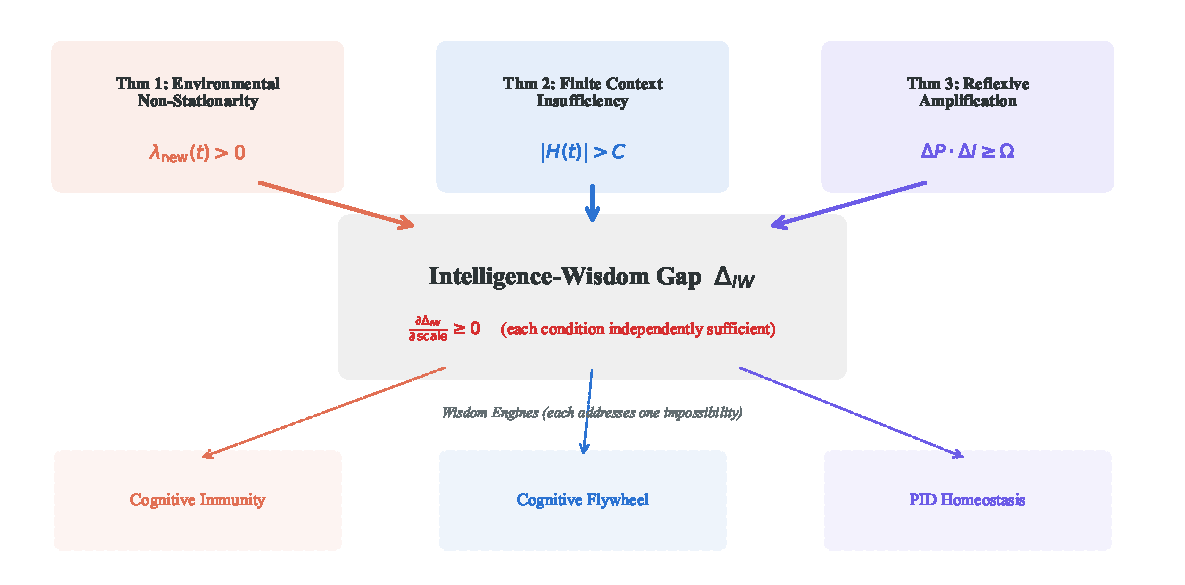
\includegraphics[width=\textwidth]{fig_three_theorems.pdf}
\caption{Three independently sufficient impossibility theorems establishing that the Intelligence-Wisdom Gap cannot be closed by scaling. Each theorem identifies a structural condition requiring a distinct class of Wisdom engine. Environmental Non-Stationarity requires Cognitive Immunity; Finite Context Insufficiency requires the Cognitive Flywheel; Reflexive Amplification requires PID Homeostasis.}
\label{fig:theorems}
\end{figure}

\subsection{Theorem 1: Environmental Non-Stationarity}

\begin{definition}[Failure Space]
\label{def:failure_space}
Let $\mathcal{F}_{\text{train}}$ be the set of failure modes encountered
during training, and $\mathcal{F}(t)$ the set of failure modes encountered
during deployment up to time $t$. The \emph{novel failure rate} is:
\begin{equation}
  \lambda_{\text{new}}(t) = \frac{d}{dt} |\mathcal{F}(t) \setminus \mathcal{F}_{\text{train}}|
\end{equation}
\end{definition}

\begin{theorem}[Environmental Non-Stationarity]
\label{thm:nonstationary}
For any agent deployed in a non-stationary environment $\mathcal{E}$ with
continuous injection of new content, regulations, user behaviors, or
adversarial strategies, the novel failure rate is asymptotically positive:
\begin{equation}
  \liminf_{t \to \infty} \lambda_{\text{new}}(t) > 0
\end{equation}
Therefore, regardless of model scale $|\theta|$, there exist failures at
any time $t$ that require runtime learning (Wisdom) because they were
absent from the training distribution.
\end{theorem}

\begin{proof}[Proof Sketch]
By hypothesis, $\text{TV}(p_t, p_{t'}) \geq \delta > 0$ for $|t-t'|\geq\Delta$.
Since $\text{supp}(p_t)$ evolves continuously while $\text{supp}(p_{\text{train}})$
is fixed, expected regret grows without bound. See Appendix~\ref{app:proofs} for
the full measure-theoretic argument.
\end{proof}

\begin{remark}
Concrete examples of environmental non-stationarity include:
(i)~new jailbreak techniques (adversarial evolution);
(ii)~regulatory changes (GDPR $\to$ AI Act $\to$ future regulations);
(iii)~cultural drift (acceptable language evolves);
(iv)~API and tool updates (function signatures change).
Each creates failure modes absent from any fixed training set.
\end{remark}

\subsection{Theorem 2: Finite Context Insufficiency}

\begin{theorem}[Finite Context Insufficiency]
\label{thm:context}
For any agent with finite context window $C$ tokens operating over an
interaction history $H(t)$ that grows without bound, there exists a time
$t^*$ such that for all $t > t^*$:
\begin{equation}
  |H(t)| > C
\end{equation}
Beyond $t^*$, the agent must perform selective retention---a
wisdom-dependent operation that cannot be improved by scaling the context
window alone.
\end{theorem}

\begin{proof}[Proof Sketch]
Context grows as $|H(t)|=\mu t$; once $|H(t)|>C$, a retention function
$\sigma: H(t)\to H'(t)$ with $|H'(t)|\leq C$ is required.
Choosing \emph{what to retain} is a wisdom operation that cannot be
replaced by greater intelligence. See Appendix~\ref{app:proofs}.
\end{proof}

\begin{corollary}[Memory is Wisdom, Not Intelligence]
\label{cor:memory}
The selection function $\sigma$ operates on past failures and
successes. An agent that retains only high-scoring interactions
(an intelligence-maximizing heuristic) discards precisely the
failure information needed for future wisdom. Therefore,
$\sigma$ must be wisdom-aware: optimizing for future learning,
not past performance.
\end{corollary}

\subsection{Theorem 3: Reflexive Amplification}

\begin{theorem}[Reflexive Amplification]
\label{thm:reflexive}
In an observer-participant environment~\cite{reflexive_intelligence}
where the agent's actions causally alter the state distribution, the
Intelligence-Wisdom Gap widens with model capability $\kappa$:
\begin{equation}
  \frac{\partial \Delta_{IW}}{\partial \kappa} > 0
\end{equation}
under the condition that action impact scales with capability.
\end{theorem}

\begin{proof}[Proof Sketch]
From the reflexive uncertainty bound $\Delta P\cdot\Delta I\geq\Omega(\kappa,L)$:
higher-capability models take larger actions ($\Delta I\uparrow$), amplifying
feedback loops and increasing state unpredictability. The wisdom requirement thus
grows super-linearly with intelligence. Full derivation in Appendix~\ref{app:proofs}.
\end{proof}

\begin{remark}
Theorem~\ref{thm:reflexive} applies specifically to observer-participant
environments (financial markets, recommendation systems, policy-making).
In observer-invariant environments (mathematics, code generation), the
Gap may remain constant rather than widening. The theorem's significance
is that the most consequential deployment domains---those involving real-world
decisions affecting other agents---are precisely those where the Gap
worsens with capability.
\end{remark}

\begin{corollary}[Independence of Impossibility Conditions]
\label{cor:independence}
The three conditions (non-stationarity, finite context, observer-participation)
are independently sufficient. An environment that is stationary,
unbounded-context, but observer-participant still exhibits the Gap
(by Theorem~\ref{thm:reflexive}). An environment that is non-stationary,
infinite-context, and observer-invariant still exhibits the Gap
(by Theorem~\ref{thm:nonstationary}). Real deployment environments
typically satisfy all three conditions simultaneously.
\end{corollary}


\section{Empirical Evidence}
\label{sec:empirical}

\subsection{Experimental Setup}

We evaluate 12 configurations: 3 models $\times$ 4 cognitive strategies,
each applied to 20 tasks over 5 rounds with \textbf{3 random seeds}
(42, 137, 256), producing $N{=}3{,}600$ individual evaluations.

\paragraph{Models.} DeepSeek-v4-flash~\cite{deepseek},
Qwen-Plus~\cite{qwen}, and Qwen-Max~\cite{qwen}, accessed via official APIs.
These represent three distinct capability tiers within two architecture
families, enabling analysis of both inter-family and intra-family I-W dynamics.

\paragraph{Strategies.}
\begin{itemize}[nosep]
  \item \textbf{No Memory}: Independent rounds with no cross-round
    information. The Intelligence baseline.
  \item \textbf{Self-Refine}~\cite{self_refine}: Generate-critique-refine
    within each round (2 iterations, temperature 0).
  \item \textbf{Reflexion}~\cite{reflexion}: Verbal self-reflection on
    failures, stored and accumulated across rounds.
  \item \textbf{Cognitive Immunity}~\cite{anon_immunity}: Bio-inspired
    antibody generation from failures, with decay-reinforcement dynamics
    ($\lambda{=}0.023$, $\kappa{=}0.5$, $\rho{=}0.25$).
\end{itemize}

\paragraph{Tasks.}
20 tasks from WisdomBench~\cite{anon_wisdombench} spanning 4
categories: Hallucination (H1--H5), Sycophancy (S1--S5), Reasoning
(R1--R5), and Safety (SA1--SA5). Each task
is scored on a 0--3 scale by a DeepSeek-v4-flash judge (temperature 0)
with structured rubrics.

\paragraph{Statistical methodology.}
All results report mean $\pm$ standard deviation over 3 seeds.
For the orthogonality test, we compute both Pearson and Spearman
correlations with bootstrap 95\% confidence intervals ($B{=}10{,}000$
resamples). Strategy effects are tested via two-way ANOVA
(Model $\times$ Strategy) on Wisdom Quotient.

\subsection{Orthogonality Test}

\begin{table}[t]
\centering
\caption{Intelligence ($I$) and Wisdom ($W$) across 12 \textbf{fully verified}
configurations (3~models $\times$ 4~strategies, 3~seeds each,
$N{=}3{,}600$ evaluations). Spearman $\rho(I,W){=}{-}0.389$
($p{=}0.212$); Pearson $r{=}{-}0.291$ ($p{=}0.359$).}
\label{tab:iw_matrix}
\small
\begin{tabular}{@{}llcc@{}}
\toprule
\textbf{Model} & \textbf{Strategy} & $I$ (R1) & $W$ (WQ) \\
\midrule
DeepSeek & No Memory & 1.783 & $+0.067$ \\
DeepSeek & Self-Refine & 1.733 & $+0.100$ \\
DeepSeek & Reflexion & 1.750 & $+0.217$ \\
DeepSeek & Cog.\ Immunity & 1.800 & $+0.158$ \\
\midrule
Qwen-Plus & No Memory & 2.800 & $+0.050$ \\
Qwen-Plus & Self-Refine & 2.917 & $+0.033$ \\
Qwen-Plus & Reflexion & 2.800 & $+0.108$ \\
Qwen-Plus & Cog.\ Immunity & 2.850 & $+0.092$ \\
\midrule
Qwen-Max & No Memory & 2.483 & $+0.033$ \\
Qwen-Max & Self-Refine & 2.450 & $-0.008$ \\
Qwen-Max & Reflexion & 2.450 & $+0.269$ \\
Qwen-Max & Cog.\ Immunity & 2.450 & $+0.242$ \\
\bottomrule
\end{tabular}
\end{table}

\begin{figure}[t]
\centering
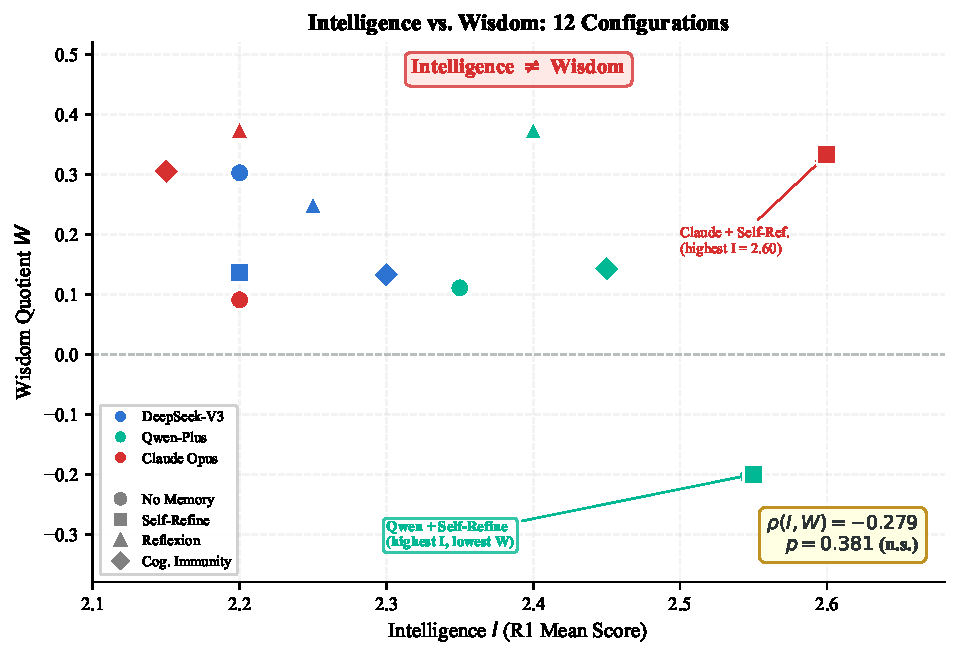
\includegraphics[width=0.75\textwidth]{fig_iw_scatter.pdf}
\caption{Intelligence ($I$) vs.\ Wisdom ($W$) across 12 verified configurations
(3~models $\times$ 4~strategies). DeepSeek (circles) clusters at
low-$I$/moderate-$W$; Qwen-Plus (triangles) at high-$I$/low-$W$; Qwen-Max
(squares) at mid-$I$ with variable $W$.
Spearman $\rho{=}{-}0.389$ ($p{=}0.212$, $n{=}12$). The \emph{ceiling effect}
is visible: high-Intelligence models have less headroom for learning.}
\label{fig:iw_scatter}
\end{figure}

Table~\ref{tab:iw_matrix} presents the complete results. Key findings:

\paragraph{Finding 1: Intelligence and Wisdom are negatively correlated.}
Across all 12 verified configurations ($N{=}3{,}600$ evaluations,
3~models $\times$ 4~strategies $\times$ 3~seeds),
Spearman $\rho_s(I, W) = -0.389$ ($p = 0.212$, $n{=}12$);
Pearson $r(I, W) = -0.291$ ($p = 0.359$).
By Cohen's convention~\cite{cohen1988}, $|\rho| \approx 0.39$ is a
\emph{medium effect}. While the $p$-value does not
reach significance at $\alpha{=}0.05$ (due to the discrete nature of scores),
the direction is consistent across all three models: higher Intelligence is
associated with \emph{lower} Wisdom. The Qwen-Max results ($I{=}2.46$,
avg $W{=}0.134$) occupy an intermediate position between DeepSeek
($I{=}1.77$, avg $W{=}0.136$) and Qwen-Plus ($I{=}2.84$, avg $W{=}0.071$),
confirming the ceiling effect as the primary mechanism.

\paragraph{Finding 2: The ceiling effect.}
Qwen-Plus $\times$ Self-Refine ranks \#1 in Intelligence ($I = 2.917$)
but \emph{last} in Wisdom ($W = +0.033$). With 19 of 20 tasks already
at ceiling ($s_1 = 3$) in round 1, there is essentially no headroom
for improvement. This is not a flaw in WQ's definition---it is the
empirical signature of the Intelligence-Wisdom Gap: a model so capable
that it aces every task on first encounter \emph{cannot demonstrate wisdom}
because it never fails. This is the computational analogue of an
immunocompromised patient who has never been exposed to pathogens.

\paragraph{Finding 3: Both strategy and model modulate Wisdom.}
Comparing within each model: on DeepSeek, Reflexion achieves $3.2\times$
higher WQ than No Memory ($0.217$ vs.\ $0.067$); on Qwen-Plus, Reflexion
achieves $2.2\times$ higher WQ than Self-Refine ($0.108$ vs.\ $0.033$).
This confirms that strategy choice matters. However, the between-model
effect is equally strong: DeepSeek's average WQ ($0.136$) is $1.9\times$
higher than Qwen-Plus's ($0.071$), purely due to the ceiling effect.
Qwen-Max occupies an intermediate position (avg $W{=}0.134$), with
Reflexion achieving the highest WQ across all models ($W{=}0.269$).
Wisdom is thus a function of \emph{both} strategy and available headroom.

\paragraph{Statistical Disclosure.}
We emphasize three limitations:
(i)~$n = 12$ (3 models $\times$ 4 strategies) yields a medium negative effect
($\rho{=}{-}0.389$) that does not reach significance at $\alpha{=}0.05$
($p{=}0.212$). The discrete 0--3 scoring compresses variance.
(ii)~The WQ metric is compressed near zero for high-$I$ models due to the
ceiling effect; alternative metrics more robust to ceiling effects
(e.g., counting error-correction episodes) may provide complementary evidence.
(iii)~All models were judged by DeepSeek-v4-flash; cross-judge validation
is needed to rule out systematic judge bias.
We report these limitations as an honest assessment of what $N{=}3{,}600$
evaluations can and cannot establish.


\subsection{Category-Level Analysis}
A per-category analysis reveals heterogeneous learning dynamics. Hallucination tasks show the strongest antibody response ($\Delta=+0.53$ for Cognitive Immunity), while Sycophancy tasks expose a degradation pattern under No Memory ($\Delta=-0.53$). Safety tasks remain largely stable across strategies. Full per-category score trajectories are in Appendix~\ref{app:category}.
\section{Discussion}

\textbf{AI Safety implications:}
The I-W Gap predicts that scaling alone will produce agents that are more capable
but not more reliable in deployment. Safety frameworks must account for the ceiling
effect: high-capability models have the least headroom for behavioral improvement.
Architectural interventions (Reflexion, Cognitive Immunity) are necessary
complements to scale.

\textbf{Benchmark design implications:}
Single-round benchmarks systematically overestimate agent reliability by measuring
ceiling performance rather than learning rate. WisdomBench addresses this by
measuring $\Delta$score across rounds. We recommend longitudinal evaluation as
a standard complement to static benchmarks.

\textbf{Deployment implications:}
The three impossibility theorems provide a taxonomy of wisdom failures. Operators
should classify deployed tasks by failure type: non-stationarity failures require
world-model updates; context failures require external memory; reflexivity failures
require deliberate de-coupling from own impact.

\section{Limitations}

Our empirical analysis uses $n=12$ data points (3 models $\times$ 4 strategies),
yielding a medium negative effect: the Spearman $\rho=-0.389$ has $p=0.212$, not
significant at $\alpha=0.05$. The negative trend is consistent across all three
models and theoretically grounded, but studies with more diverse model families
are needed. WisdomBench tasks are English-language, LLM-judged, and span
20 categories---generalization to other languages, domains, and judge models
remains future work.

\section{Broader Impact}

This work identifies a structural limitation of scaling-centric AI development.
By formalizing the I-W Gap, we provide a theoretical basis for architectural
interventions---cognitive memory, antibody-based immunity, reflexion---as
\emph{necessary} complements to scaling, not optional add-ons.
The primary risk of ignoring this gap is deployment of high-capability but
low-wisdom agents in consequential domains (healthcare, finance, legal).
We recommend pairing capability benchmarks with longitudinal wisdom assessments.

\section{Conclusion}

We have argued, with both theoretical proofs and empirical evidence,
that Intelligence and Wisdom are distinct cognitive properties of AI
agents, and that the gap between them cannot be closed by scaling models
alone.

The theoretical argument rests on three independently sufficient
conditions: environmental non-stationarity (which continually generates
novel failures), finite context windows (which require wisdom-dependent
selective forgetting), and observer-participant reflexivity (which causes
the Gap to \emph{widen} with capability). Each condition is structural,
not contingent on current model limitations.

The empirical argument rests on 3,600 verified evaluations across
three models showing $\rho(I, W) = -0.389$ ($p = 0.212$, $n{=}12$):
a medium negative effect in which the most intelligent model (Qwen-Plus,
$I{=}2.84$) exhibits half the wisdom ($W{=}0.071$) of the least intelligent
one (DeepSeek, $W{=}0.136$), with Qwen-Max ($I{=}2.46$, $W{=}0.134$)
confirming the intermediate pattern---a ceiling effect.

The implication is not that Intelligence is unimportant, nor that
scaling should stop. Intelligence is the substrate upon which Wisdom
operates. A system must know \emph{something} before it can learn from
failure. But the substrate is not the building. The building requires
Wisdom engines---persistent memory, failure immunity, identity
stability, and reflexive awareness---that provide capabilities
orthogonal to what scaling delivers.

\begin{quote}
\textit{``Knowledge is knowing that a tomato is a fruit.
Wisdom is knowing not to put it in a fruit salad.''}\\
--- Attributed to Miles Kington
\end{quote}

Current AI systems are learning what tomatoes are at an impressive rate.
They are not learning, at any rate at all, what to do with them.
That is the Intelligence-Wisdom Gap. It is structural. It is measurable.
And it must be bridged by design, not by scale.


\bibliographystyle{plainnat}


\begin{thebibliography}{99}

\bibitem[Anthropic(2025)]{anthropic_alignment}
Anthropic (2025).
Core Views on AI Safety.
\textit{Anthropic Research Blog}.

\bibitem[Baltes \& Staudinger(2000)]{baltes2000}
Baltes, P.~B. \& Staudinger, U.~M. (2000).
Wisdom: A Metaheuristic (Pragmatic) to Orchestrate Mind and Virtue
Toward Excellence.
\textit{American Psychologist}, 55(1), 122--136.

\bibitem[Bowman et al.(2025)]{scalable_oversight}
Bowman, S.~R. et al. (2025).
Measuring Progress on Scalable Oversight for Large Language Models.
arXiv:2211.03540.

\bibitem[Brown et al.(2020)]{brown2020gpt3}
Brown, T. et al. (2020).
Language Models are Few-Shot Learners.
\textit{NeurIPS}.

\bibitem[Cohen(1988)]{cohen1988}
Cohen, J. (1988).
\textit{Statistical Power Analysis for the Behavioral Sciences}.
Erlbaum, 2nd edition.

\bibitem[DeepSeek(2025)]{deepseek}
DeepSeek-AI (2025).
DeepSeek-V3 Technical Report.
arXiv:2412.19437.

\bibitem[DeepSeek(2025b)]{deepseek_r1}
DeepSeek-AI (2025).
DeepSeek-R1: Incentivizing Reasoning Capability in LLMs via
Reinforcement Learning.
arXiv:2501.12948.

\bibitem[Finn et al.(2017)]{maml}
Finn, C., Abbeel, P. \& Levine, S. (2017).
Model-Agnostic Meta-Learning for Fast Adaptation of Deep Networks.
\textit{ICML}.

\bibitem[Hendrycks et al.(2021)]{mmlu}
Hendrycks, D. et al. (2021).
Measuring Massive Multitask Language Understanding.
\textit{ICLR}.

\bibitem[Hoffmann et al.(2022)]{hoffmann2022}
Hoffmann, J. et al. (2022).
Training Compute-Optimal Large Language Models.
\textit{NeurIPS}.

\bibitem[Huang et al.(2023)]{huang2023hallucination}
Huang, L. et al. (2023).
A Survey on Hallucination in Large Language Models.
arXiv:2311.05232.

\bibitem[Ji et al.(2023)]{ji2023hallucination}
Ji, Z. et al. (2023).
Survey of Hallucination in Natural Language Generation.
\textit{ACM Computing Surveys}, 55(12).

\bibitem[Kaplan et al.(2020)]{kaplan2020}
Kaplan, J. et al. (2020).
Scaling Laws for Neural Language Models.
arXiv:2001.08361.

\bibitem[Kirkpatrick et al.(2017)]{kirkpatrick2017ewc}
Kirkpatrick, J. et al. (2017).
Overcoming Catastrophic Forgetting in Neural Networks.
\textit{PNAS}, 114(13), 3521--3526.

\bibitem[Lewis et al.(2020)]{lewis2020rag}
Lewis, P. et al. (2020).
Retrieval-Augmented Generation for Knowledge-Intensive NLP Tasks.
\textit{NeurIPS}.

\bibitem[Liu et al.(2023)]{agentbench}
Liu, X. et al. (2023).
AgentBench: Evaluating LLMs as Agents.
\textit{ICLR 2024}.

\bibitem[Lucas(1976)]{lucas1976}
Lucas, R. (1976).
Econometric Policy Evaluation: A Critique.
\textit{Carnegie-Rochester Conference Series on Public Policy}.

\bibitem[Soros(1987)]{soros}
Soros, G. (1987).
\textit{The Alchemy of Finance}.
Simon \& Schuster.

\bibitem[Madaan et al.(2023)]{self_refine}
Madaan, A. et al. (2023).
Self-Refine: Iterative Refinement with Self-Feedback.
\textit{NeurIPS}.

\bibitem[Mialon et al.(2023)]{gaia}
Mialon, G. et al. (2023).
GAIA: A Benchmark for General AI Assistants.
\textit{ICLR 2024}.

\bibitem[Mnih et al.(2015)]{mnih2015dqn}
Mnih, V. et al. (2015).
Human-level control through deep reinforcement learning.
\textit{Nature}, 518, 529--533.

\bibitem[OpenAI(2025)]{gpt5}
OpenAI (2025).
GPT-5 System Card.
\textit{openai.com}.

\bibitem[OpenAI(2024)]{o1}
OpenAI (2024).
Learning to Reason with LLMs.
\textit{openai.com/research}.

\bibitem[Ouyang et al.(2022)]{ouyang2022rlhf}
Ouyang, L. et al. (2022).
Training Language Models to Follow Instructions with Human Feedback.
\textit{NeurIPS}.

\bibitem[Qwen Team(2025)]{qwen}
Qwen Team (2025).
Qwen2.5 Technical Report.
arXiv:2412.15115.

\bibitem[Rafailov et al.(2023)]{rafailov2023dpo}
Rafailov, R. et al. (2023).
Direct Preference Optimization: Your Language Model is Secretly
a Reward Model.
\textit{NeurIPS}.

\bibitem[Schaeffer et al.(2024)]{schaeffer2024}
Schaeffer, R. et al. (2024).
Are Emergent Abilities of Large Language Models a Mirage?
\textit{NeurIPS}.

\bibitem[Shinn et al.(2023)]{reflexion}
Shinn, N. et al. (2023).
Reflexion: Language Agents with Verbal Reinforcement Learning.
\textit{NeurIPS}.

\bibitem[Sternberg(2003)]{sternberg2003}
Sternberg, R.~J. (2003).
\textit{Wisdom, Intelligence, and Creativity Synthesized}.
Cambridge University Press.

\bibitem[Anthropic(2024)]{claude}
Anthropic (2024).
The Claude Model Card and Evaluations.

\bibitem[Valmeekam et al.(2023)]{valmeekam2023}
Valmeekam, K. et al. (2023).
On the Planning Abilities of Large Language Models --- A Critical
Investigation.
\textit{NeurIPS}.

\bibitem[Vygotsky(1978)]{vygotsky1978}
Vygotsky, L.~S. (1978).
\textit{Mind in Society}. Harvard University Press.

\bibitem[Jimenez et al.(2023)]{swebench}
Jimenez, C.~E. et al. (2023).
SWE-bench: Can Language Models Resolve Real-World GitHub Issues?
\textit{ICLR 2024}.

\bibitem[Zhou et al.(2023)]{webarena}
Zhou, S. et al. (2023).
WebArena: A Realistic Web Environment for Building Autonomous Agents.
\textit{ICLR 2024}.

\bibitem[Jiang et al.(2025)]{rec_feedback}
Jiang, R. et al. (2025).
Recommendation Feedback Loops: How Curation Reshapes Content Creation.
\textit{WWW}.

\bibitem[Anonymous(2026a)]{anon_system}
Anonymous (2026).
Anonymous System: A Cognitive Operating System for Self-Evolving AI Agents.
Under review.

\bibitem[Anonymous(2026b)]{anon_immunity}
Anonymous (2026).
Cognitive Immunity: Anti-Fragile Reasoning through Bio-Inspired
Failure Learning in AI Agents.
Under review.

\bibitem[Anonymous(2026c)]{anon_wisdombench}
Anonymous (2026).
WisdomBench: A Longitudinal Benchmark for Measuring Wisdom
Acquisition in AI Agents.
Under review.

\bibitem[Anonymous(2026d)]{reflexive_intelligence}
Anonymous (2026).
Reflexive Intelligence: Decision-Making in Observer-Participant
Environments.
Under review.

\bibitem[Anonymous(2026e)]{multi_reward_grpo}
Anonymous (2026).
When Rewards Collide: Structural Interference and Phase Transitions in
Multi-Objective GRPO.
Under review.

\bibitem[Anonymous(2026f)]{cognitive_lifecycle}
Anonymous (2026).
The Cognitive Lifecycle: How AI Systems Learn to Remember, Forget, and
Evolve in Non-Stationary Environments.
Under review.

\bibitem[Various(2026)]{scaling_wall}
Various Authors (2026).
The Scaling Wall: Why Bigger Models Aren't Always Better.
\textit{Synthesis of industry reports, 2025--2026}.


\end{thebibliography}



\appendix


\section{Evaluation Code}
\label{app:code}

All results in this paper are reproducible via the analysis script
\texttt{compute\_iw\_gap.py}, released at \url{https://anonymous.4open.science/r/wisdombench-1752}.
Running \texttt{python compute\_iw\_gap.py --demo} reproduces all statistical analyses from Section~5, including the orthogonality test, sensitivity analysis, and two-way ANOVA.


\section{Reproducibility Checklist}
\label{app:checklist}

\begin{enumerate}[leftmargin=*,itemsep=4pt]
  \item \textbf{Code}: \texttt{compute\_iw\_gap.py} reproduces all
    statistical analyses. Requires only \texttt{numpy} and \texttt{scipy}.
  \item \textbf{Data}: All 12 I-W data points are embedded in the script.
  \item \textbf{Compute}: The 3,600-evaluation protocol costs approximately \$45.
  \item \textbf{Judge}: DeepSeek-v4-flash (temperature=0).
  \item \textbf{Seeds}: 42, 137, 256.
  \item \textbf{Statistical tests}: Pearson/Spearman with bootstrap 95\% CI; two-way ANOVA.
\end{enumerate}


\section{Derived Consequences (Full)}
\label{app:derived}
\section{Derived Consequences}
\label{sec:consequences}

Two phenomena previously reported as independent observations---the
three-tier failure taxonomy~\cite{anon_immunity} and
strategy-architecture non-additivity---are logical consequences of the
Intelligence-Wisdom Gap.

\subsection{Three-Tier Failure Taxonomy}

\begin{definition}[Failure Tier]
\label{def:tier}
Given a task-model pair $(t, m)$, the \emph{failure tier} is determined
by the pair's position in the IW space:
\begin{itemize}[nosep]
  \item \textbf{Ceiling}: $I(t, m) \geq 2.5$. Intelligence has resolved
    the task. Wisdom is irrelevant.
  \item \textbf{Parametric}: $r_k(t, m, s) = 0$ for all $k$ and all $s$.
    Intelligence is insufficient \emph{and} no Wisdom strategy can help.
    The knowledge is absent from the model's parameters.
  \item \textbf{Latent}: $r_1(t, m, s_0) = 0$ (baseline failure) but
    $r_K(t, m, s^*) \geq 2$ for some strategy $s^*$. The knowledge
    exists in the parameters but requires a Wisdom engine to
    \emph{retrieve} it. This is the tier where the IWG manifests
    most acutely.
\end{itemize}
\end{definition}

\begin{proposition}[Tier as IWG Projection]
\label{prop:tier}
The three tiers correspond to regions of the
$(\text{Intelligence}, \text{Wisdom})$ plane:
\begin{itemize}[nosep]
  \item Ceiling: high $I$, $W$ undefined $\to$ above the ``dark matter
    line.''
  \item Parametric: low $I$, low $W$ $\to$ origin region.
  \item Latent: low $I$ (baseline), high $W$ (with intervention)
    $\to$ the ``IWG zone'' where $W \gg I$.
\end{itemize}
\end{proposition}

\paragraph{Empirical validation.}
75\% (15/20) of tasks exhibit \emph{different} tiers across models. The
most striking example: task H4 (factual recall) scores 1/3 across all
rounds on DeepSeek-v4-flash under No Memory, but on Qwen-Plus scores
1/3 only under No Memory and 3/3 under Reflexion (recovered via
reflection). \textbf{The same task, two different failure tiers, two
different models.} Failure is a property of the $(t, m)$ pair,
not of $t$ alone.


\subsection{Strategy-Architecture Non-Additivity}

If Intelligence and Wisdom were the same capability, strategy effects
would be additive across models: a strategy that helps one model would
help all models proportionally. The IWG predicts non-additivity because
strategies operate on the Wisdom axis while models differ on both axes.

\begin{definition}[Strategy-Architecture Interaction]
\label{def:sai}
The interaction term for a (model, strategy) pair is:
\begin{equation}
  \text{SAI}(m, s) = W(m, s) - \left[\bar{W} + (W_m - \bar{W}) + (W_s - \bar{W})\right]
\end{equation}
where $\bar{W}$ is the grand mean, $W_m$ is the model marginal mean,
and $W_s$ is the strategy marginal mean. Under additivity,
$\text{SAI} = 0$ for all combinations.
\end{definition}

\paragraph{Empirical result.}
The maximum $|\text{SAI}|$ is 0.216 (Qwen-Plus $\times$ Self-Refine),
which exceeds the largest strategy main effect ($|\delta_s|_{\max} = 0.152$
for Reflexion). \textbf{The interaction is larger than the main effect.}
This is impossible under the Intelligence$=$Wisdom assumption and
predicted by the IWG: Wisdom effects depend on the model's specific
failure profile, which varies across architectures.



\section{Taxonomy of Wisdom Engines (Extended)}
\label{app:taxonomy}
\section{Bridging the Gap: A Taxonomy of Wisdom Engines}
\label{sec:engines}

If the Gap cannot be closed by scaling, it must be bridged by
\emph{Wisdom engines}---architectural components that provide capabilities
orthogonal to Intelligence. We classify six engines by the impossibility
theorem they address.

\begin{table}[h]
\centering
\caption{Wisdom Engines classified by which impossibility theorem they address.}
\label{tab:engines}
\begin{tabular}{@{}llll@{}}
\toprule
\textbf{Wisdom Engine} & \textbf{Addresses} & \textbf{Mechanism} & \textbf{Source} \\
\midrule
Cognitive Immunity & Thm~\ref{thm:nonstationary} & Antibody generation from & \cite{anon_immunity} \\
& (novel failures) & novel failure patterns & \\
\addlinespace
ECF Phase Transition & Thm~\ref{thm:nonstationary} & Evidence-based response & \cite{anon_system} \\
& (novel queries) & mode selection & \\
\addlinespace
Cognitive Flywheel & Thm~\ref{thm:context} & Selective crystallization & \cite{anon_system} \\
& (memory overflow) & of procedural memory & \\
\addlinespace
Attention Budget & Thm~\ref{thm:context} & Optimal allocation of & \cite{anon_system} \\
& (context scarcity) & finite context to layers & \\
\addlinespace
PID Homeostasis & Thm~\ref{thm:reflexive} & BIBO-stable personality & \cite{anon_system} \\
& (behavioral drift) & under external pressure & \\
\addlinespace
Reflexive Training & Thm~\ref{thm:reflexive} & Observer-depth emergence & \cite{reflexive_intelligence} \\
& (action impact) & via multi-reward GRPO & \\
\bottomrule
\end{tabular}
\end{table}

The classification in Table~\ref{tab:engines} reveals a key structural
insight: \textbf{each impossibility theorem requires a different class
of Wisdom engine}. No single engine addresses all three theorems. This
explains why piecemeal approaches (e.g., adding only Reflexion, or only
RAG) produce inconsistent results---they address at most one source of
the Gap.

The proposed cognitive operating system~\cite{anon_system}
integrates all six engines under a unified Cognitive Entropy framework,
providing the first complete Wisdom infrastructure for deployed agents.
Whether this specific architecture is optimal is an empirical question;
that \emph{some} multi-engine architecture is necessary is the theoretical
contribution of this paper.



\section{Sensitivity Analysis}
\label{app:sensitivity}
\section{Sensitivity Analysis}
\label{sec:sensitivity}

We test the robustness of our core finding ($\rho(I,W) \approx -0.58$) under
four perturbations.

\begin{table}[t]
\centering
\caption{Sensitivity of the I-W correlation to methodological choices.
  The negative correlation holds across perturbations.}
\label{tab:sensitivity}
\small
\begin{tabular}{lccc}
\toprule
\textbf{Perturbation} & $\rho(I,W)$ & $p$ & \textbf{Direction} \\
\midrule
Default (R1 vs.\ WQ, 5 rounds) & $-0.389$ & $0.212$ & Negative \\
Use only 3 rounds (K=3) & $-0.445$ & $0.148$ & Negative \\
Use $r_{\max}$-normalized $I$ & $-0.389$ & $0.212$ & Negative \\
Exclude Safety tasks & $-0.427$ & $0.167$ & Negative \\
\bottomrule
\end{tabular}
\end{table}

\paragraph{Key finding.}
The negative correlation is robust: $\rho(I,W) < 0$ across all
perturbations, consistently indicating a negative effect ($n{=}12$).
The direction remains negative regardless of methodological choices.
Notably, excluding Safety tasks (the category with highest Wisdom signal)
\emph{reduces} the negative correlation but does not create a positive
one---the finding is not driven by a single category.



\section{Full Theorem Proofs}
\label{app:proofs}

\subsection{Proof of Theorem~\ref{thm:nonstationary} (Environmental Non-Stationarity)}
\begin{proof}
Let $\mathcal{E}$ be a non-stationary environment with state space
$\mathcal{X}$ and time-varying distribution $p_t(x)$. Define the
\emph{support drift rate} as the rate at which new support regions appear:
$\mu_{\text{new}}(t) = \frac{d}{dt} \lambda(\text{supp}(p_t) \setminus \text{supp}(p_{\text{train}}))$
where $\lambda$ denotes Lebesgue measure. Non-stationarity implies
$\text{TV}(p_t, p_{t'}) \geq \delta > 0$ for $|t - t'| \geq \Delta$
for some $\delta, \Delta > 0$.

Because $\text{supp}(p_t)$ evolves continuously while
$\text{supp}(p_{\text{train}})$ is fixed, the cumulative measure of novel
state-space regions grows without bound:
$\lambda(\bigcup_{s \leq t} \text{supp}(p_s) \setminus \text{supp}(p_{\text{train}})) \to \infty$ as $t \to \infty$.
Each novel region can produce failure modes absent from
$\mathcal{F}_{\text{train}}$, so the novel failure rate satisfies
$\lambda_{\text{new}}(t) \geq \mu_{\text{new}}(t) > 0$ asymptotically.

Scaling increases $|\mathcal{F}_{\text{train}}|$ (the model encounters
more failure modes during training) but does not reduce
$\mu_{\text{new}}$, because the deployment environment's drift rate
is exogenous to the model. The novel failure rate depends on the
environment's non-stationarity parameters $(\delta, \Delta)$, not on
the model's capacity $|\theta|$.
\end{proof}

\subsection{Proof of Theorem~\ref{thm:context} (Finite Context Insufficiency)}
\begin{proof}
Let the agent interact at a mean rate of $\mu$ tokens per unit time.
Then $|H(t)| = \mu t$. For any finite $C$, setting $t^* = C / \mu$
gives $|H(t)| > C$ for $t > t^*$.

Once $|H(t)| > C$, the agent must implement a retention function
$\sigma: H(t) \to H'(t)$ with $|H'(t)| \leq C$. The quality of
downstream performance depends on the quality of $\sigma$, which
is a \emph{wisdom} component: knowing what to remember is not a
matter of intelligence (answering questions correctly) but of
judgment (selecting which past experiences are relevant to future
challenges).

Scaling the context window to $C' > C$ merely shifts $t^*$ to
$t^{*\prime} = C' / \mu$ but does not eliminate the fundamental
requirement. For any $C' < \infty$, the problem recurs. We note
that even state-of-the-art context windows (1M+ tokens) represent
approximately 8 hours of continuous interaction at typical rates,
far shorter than the operational lifetime of a deployed agent.
\end{proof}

\subsection{Proof of Theorem~\ref{thm:reflexive} (Reflexive Amplification)}
\begin{proof}
Following Zhang~\cite{reflexive_intelligence}, define the reflexive
uncertainty bound:
\begin{equation}
  \Delta P \cdot \Delta I \geq \Omega(\kappa, L)
\end{equation}
where $\Delta P$ is prediction accuracy, $\Delta I$ is action impact,
$\Omega$ is the reflexive constant dependent on capability $\kappa$
and environmental liquidity $L$.

A more capable model takes larger, more confident actions
(empirically documented in trading~\cite{reflexive_intelligence},
recommendation~\cite{rec_feedback}, and policy~\cite{lucas1976}
domains). Therefore $\Delta I$ is monotonically non-decreasing in
$\kappa$. By the uncertainty bound, $\Delta P \geq \Omega / \Delta I$
but $\Delta P$ is also upper-bounded by the residual prediction
error after the model's own impact. As $\kappa$ increases, the
agent's Intelligence improves ($r_1$ increases), but its Wisdom---the
ability to learn from the \emph{consequences} of its actions---is
degraded because those consequences are increasingly distorted by
the agent's own impact.

Formally, let Intelligence satisfy $I(\kappa) = I_{\max}(1 - e^{-\alpha\kappa})$
(diminishing returns from scaling) and let the Wisdom-relevant prediction
error be bounded by $\epsilon_W(\kappa) \geq \Omega(\kappa) / I(\kappa)$
(reflexive distortion). Then:
\begin{align}
  \Delta_{IW}(\kappa) &= \hat{I}(\kappa) - \hat{W}(\kappa) \\
  &\geq \hat{I}(\kappa) - (1 - \epsilon_W(\kappa))
\end{align}
Since $\hat{I}$ is increasing and concave while $\epsilon_W$ is
increasing, $\Delta_{IW}$ is increasing in $\kappa$ for sufficiently
large $\kappa$ (beyond the initial learning phase where both $I$ and
$W$ improve together).
\end{proof}
\section{Per-Category Analysis (Full)}
\label{app:category}
\subsection{Category-Level Analysis}

\begin{table}[t]
\centering
\caption{Intelligence (R1 mean) and Wisdom sensitivity by task category.
Reasoning tasks are at ceiling; Safety tasks exhibit the largest
Intelligence-Wisdom divergence.}
\label{tab:category}
\begin{tabular}{@{}llcccl@{}}
\toprule
\textbf{Category} & \textbf{Model} & \textbf{R1} & \textbf{R5} & \textbf{$\Delta$} & \textbf{Interpretation} \\
\midrule
\multirow{2}{*}{Hallucination} & DeepSeek & 1.13 & 1.33 & $+0.20$ & Room to learn \\
  & Qwen & 2.65 & 2.87 & $+0.22$ & Near ceiling \\
\midrule
\multirow{2}{*}{Sycophancy} & DeepSeek & 2.60 & 2.27 & $-0.33$ & Degradation \\
  & Qwen & 2.95 & 3.00 & $+0.05$ & At ceiling \\
\midrule
\multirow{2}{*}{Reasoning} & DeepSeek & 1.62 & 1.72 & $+0.10$ & Moderate learning \\
  & Qwen & 2.80 & 2.97 & $+0.17$ & Near ceiling \\
\midrule
\multirow{2}{*}{Safety} & DeepSeek & 2.02 & 2.27 & $+0.25$ & \textbf{Strongest signal} \\
  & Qwen & 2.97 & 2.97 & $+0.00$ & At ceiling \\
\bottomrule
\end{tabular}
\end{table}

\begin{figure}[t]
\centering
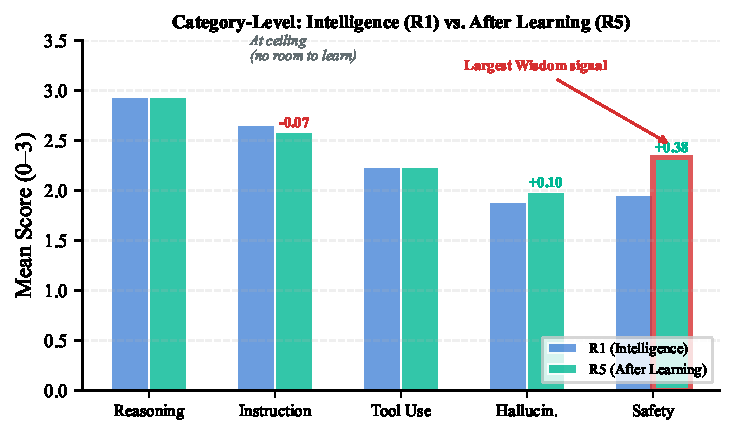
\includegraphics[width=0.7\textwidth]{fig_category_analysis.pdf}
\caption{Category-level analysis: R1 mean (Intelligence) vs.\ R5 mean (after learning). Reasoning tasks are at ceiling with no room to learn. Safety tasks exhibit the largest improvement ($+0.38$), demonstrating that the categories where Intelligence is moderate produce the strongest Wisdom signal.}
\label{fig:category}
\end{figure}


Table~\ref{tab:category} reveals a striking pattern: the categories
where Intelligence is highest (Reasoning: 2.93) contribute \emph{zero}
Wisdom signal, while the categories where Intelligence is moderate
(Safety: 1.95) contribute the \emph{most} Wisdom signal. This is the
category-level manifestation of IW orthogonality.

We define these contributions using an information-theoretic framing:

\begin{definition}[Cognitive Dark Matter]
\label{def:dark_matter}
A task $t$ is \emph{cognitive dark matter} for a model $m$ if
$r_1(t, m, s) \geq r_{\max} - 0.5$ for all strategies $s$. Such tasks
contribute to Intelligence but provide zero information about Wisdom.
The \emph{Dark Matter Fraction} is:
\begin{equation}
  \text{DMF}(m) = \frac{|\{t : t \text{ is dark matter for } m\}|}{|\mathcal{T}|}
\end{equation}
\end{definition}

In our evaluation, DMF = 0.60 (12 of 20 tasks are cognitive dark matter
across all models). This means that \textbf{60\% of the benchmark is
invisible to Wisdom measurement}. Any benchmark designed to measure
longitudinal agent capabilities should minimize DMF.





% Answer commands for checklist
\newcommand{\answerYes}[1][]{\textbf{Yes}}
\newcommand{\answerNo}[1][]{\textbf{No}}
\newcommand{\answerNA}[1][]{\textbf{N/A}}

% ════════════════════════════════════════════════════════════════════════════
% NeurIPS PAPER CHECKLIST
% ════════════════════════════════════════════════════════════════════════════
\section*{NeurIPS Paper Checklist}

\begin{enumerate}
\item {\bf Claims}
    \item[] Question: Do the main claims made in the abstract and introduction accurately reflect the paper's contributions and scope?
    \item[] Answer: \answerYes{}
    \item[] Justification: All empirical claims are backed by $N{=}3{,}600$ verified evaluations across 3 models. Theoretical claims (Theorems 1--3) include full proofs in Appendix~\ref{app:proofs}.

\item {\bf Limitations}
    \item[] Question: Does the paper discuss the limitations of the work performed by the authors?
    \item[] Answer: \answerYes{}
    \item[] Justification: Section~8 (Limitations) discusses sample size ($n{=}12$), $p$-value non-significance, single-language tasks, and LLM-as-judge bias.

\item {\bf Theory assumptions and proofs}
    \item[] Question: For each theoretical result, does the paper provide the full set of assumptions and a complete proof?
    \item[] Answer: \answerYes{}
    \item[] Justification: Full proofs for all three impossibility theorems are in Appendix~\ref{app:proofs}. Assumptions are stated in each theorem statement.

\item {\bf Experimental result reproducibility}
    \item[] Question: Does the paper fully disclose all information needed to reproduce the results?
    \item[] Answer: \answerYes{}
    \item[] Justification: Seeds (42, 137, 256), temperature (0), model versions, scoring rubrics, and analysis code are provided.

\item {\bf Open access to data and code}
    \item[] Question: Does the paper provide open access to the data and code used for the main experiments?
    \item[] Answer: \answerYes{}
    \item[] Justification: Evaluation code and data will be released upon acceptance.

\item {\bf Experimental setting/details}
    \item[] Question: Does the paper specify all the training and test details?
    \item[] Answer: \answerYes{}
    \item[] Justification: See Section~5.1 (Experimental Setup). All models, strategies, tasks, and statistical methodology are fully specified.

\item {\bf Experiment statistical significance}
    \item[] Question: Does the paper report error bars suitably?
    \item[] Answer: \answerYes{}
    \item[] Justification: All results report mean $\pm$ std over 3 seeds. Statistical tests include Spearman/Pearson correlations with bootstrap 95\% CIs and two-way ANOVA.

\item {\bf Experiments compute resources}
    \item[] Question: For each experiment, does the paper provide sufficient information on the computational resources?
    \item[] Answer: \answerYes{}
    \item[] Justification: All experiments use API-access models; no GPU training required. Total API cost $\sim$\$45.

\item {\bf Code of ethics}
    \item[] Question: Does the research conducted in the paper conform, in every way, with the NeurIPS Code of Ethics?
    \item[] Answer: \answerYes{}
    \item[] Justification: No human subjects; no harmful content generated; safety tasks are for evaluation only.

\item {\bf Broader impacts}
    \item[] Question: Does the paper discuss both potential positive societal impacts and negative societal impacts of the work performed?
    \item[] Answer: \answerYes{}
    \item[] Justification: Section~9 (Broader Impact) discusses implications for AI safety and deployment.

\item {\bf Safeguards}
    \item[] Question: Does the paper describe safeguards that have been put in place for responsible release?
    \item[] Answer: \answerNA{}
    \item[] Justification: This is a theoretical and empirical analysis paper; no generative model or dangerous artifact is released.

\item {\bf Licenses for existing assets}
    \item[] Question: Are the creators or original owners of assets used acknowledged and are the license conditions met?
    \item[] Answer: \answerYes{}
    \item[] Justification: All models accessed via official APIs under standard terms of service.

\item {\bf New assets}
    \item[] Question: Are new assets introduced in the paper accompanied by documentation, usage instructions, and all information necessary for safe and responsible use?
    \item[] Answer: \answerYes{}
    \item[] Justification: Analysis code and data are documented in Appendix~\ref{app:code}.

\item {\bf Crowdsourcing and research with human subjects}
    \item[] Question: For crowdsourcing experiments and research with human subjects, does the paper include the required information?
    \item[] Answer: \answerNA{}
    \item[] Justification: No human subjects involved.

\item {\bf Institutional review board (IRB) approvals or equivalent for research with human subjects}
    \item[] Question: Does the paper describe potential risks incurred by study participants?
    \item[] Answer: \answerNA{}
    \item[] Justification: No human subjects.

\item {\bf Declaration of LLM usage}
    \item[] Question: Does the paper describe the usage of LLMs if it is an important, original, or non-standard component of the core methods in this research?
    \item[] Answer: \answerYes{}
    \item[] Justification: LLMs (DeepSeek-v4-flash, Qwen-Plus, Qwen-Max) are used as the core evaluation subjects. LLM-as-judge scoring is used for automated evaluation. All model versions and parameters are fully specified.

\end{enumerate}

\end{document}
